\chapter{Modeling of processes in \texorpdfstring{\ce{CO2}}{CO2} amplifiers}\label{chapter:models}


\section{Basics of the molecular spectroscopy of \ce{CO2}}

\subsection{Isotopologues of \ce{CO2} and their nomenclature}

The \textbf{\texttt{co2amp}} model includes twelve isotopologues of \ce{CO2} with different combinations of stable isotopes of carbon (\ce{^{12}C} and \ce{^{13}C}) and oxygen (\ce{^{16}O}, \ce{^{17}O} and \ce{^{18}O}). A commonly used three-digit notation designates the isotopologues of carbon dioxide, where each digit represents the isotope of an atom in the molecule in the order oxygen–carbon–oxygen, corresponding to the last digit of the isotope's mass number. In this notation, the digits \textit{2} and \textit{3} represent \ce{^{12}C} and \ce{^{13}C}, respectively, while the digits \textit{6}, \textit{7} and \textit{8} represent \ce{^{16}O}, \ce{^{17}O} and \ce{^{18}O}, respectively. Thus, \textit{626}, for instance, denotes a \ce{CO2} molecule with the natural isotopic composition \ce{^{16}O}-\ce{^{12}C}-\ce{^{16}O}, and \textit{638} stands for the \ce{^{16}O}-\ce{^{13}C}-\ce{^{18}O} isotopologue.




\subsection{Vibrational levels of \ce{CO2} molecule}

\subsubsection{Laser transitions}

Laser transitions in \ce{CO2} amplifiers occur between the rotational sub-levels of vibrational levels in the electronic ground state of the molecule. The primary laser transitions (''Regular bands'') are between the first excited state of the antisymmetric stretching vibration and one of the combination vibrations involving the first excited state of the symmetric stretching and the second excited state of the bending vibration. However, transitions between higher energy levels are also possible, potentially contributing to the overall gain of the amplifier. Multiple vibrational energy levels are thus included in the \textbf{\texttt{co2amp}} amplification model. Figure~\ref{fig:laser-transitions} shows some of the laser transitions included in the \textbf{\texttt{co2amp}} amplification model and the vibrational levels involved in these transitions.

\begin{figure}[ht]
\centering
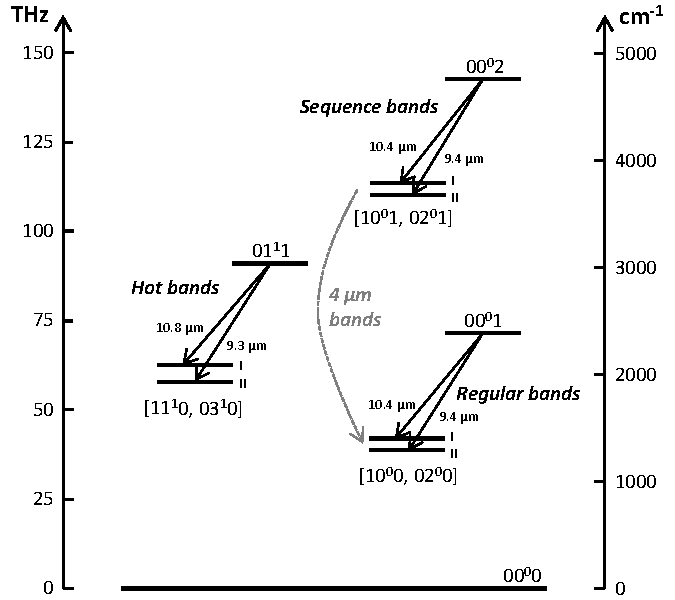
\includegraphics[width=120mm]{images/laser-transitions}
\caption{Vibrational transitions included in the amplification model. Wavelengths are given for natural \ce{CO2} isotopologue (\textit{626}).}\label{fig:laser-transitions}
\end{figure}

Other vibrational levels contributing to the population dynamics of the laser levels are not shown in the figure but are included in the model as described in the following text. Additionally, the code includes experimental support for modeling laser transitions at approximately \SI{4}{\micro\meter} between the group of levels at the end of the sequence bands and the group of levels including the lower levels of the regular bands. Below, we describe the basics of the involved molecular spectroscopy, followed by the description of the model of the population dynamics and stimulated emission.



\subsubsection{Vibrational level nomenclature}

A standard scheme of vibrational level nomenclature uses the $\nu_1\,\nu_2^{l[e/f]}\,\nu_3$ notation, where $\nu_1$, $\nu_2$, and $\nu_3$ are the numbers of quanta in the symmetric stretch, bending, and antisymmetric stretch vibrational modes, respectively, and $l$ is the vibrational angular momentum quantum number of the doubly degenerate bending vibration. States with $l \neq 0$ are further split into two sub-levels due to the two possible symmetries associated with the bending vibration. A letter $e$ or $f$ is added to the notation after the value of $l$ to differentiate between these sub-levels.

In the \ce{CO_2} molecule, a strong Fermi coupling exists between the $\nu_1$ and $\nu_2$ vibrations, resulting in mixed states that cannot be directly attributed to a single set of vibrational quantum numbers. We refer to these levels by listing the contributing states in square brackets and adding a Roman numeral subscript indicating a sub-level number. For instance, the lower laser level of the \SI{9.4}{\micro\meter} regular band is denoted as $[1\,0^{0}0,\,0\,2^{0}0]_{\mathrm{II}}$.

In the HITRAN database, the symmetry of the bending vibration ($e$ or $f$) is associated with the rotational levels rather than with the vibrational ones, as in the \textbf{\texttt{co2amp}} model. Associating the symmetry with the vibrational state makes modeling the energy distribution between ro-vibrational sub-levels more straightforward and transparent. Also, the letter $e$ is associated with the $l = 0$ levels in HITRAN for database consistency.

Furthermore, in HITRAN, the mixed states are labeled by one of the contributing states followed by a sub-level number. The $[1\,0^{0}0,\,0\,2^{0}0]_{\mathrm{II}}$ level, for example, is denoted as $1\,0^{0}0\,(2)$ (or $1\,0\,0\,0\,2$ in the raw \texttt{.par} files). The letter $e$ is then added to the rotational level labels (e.g., ''P 20e'').




\subsubsection{Vibrational levels and transitions included in the \textbf{\texttt{co2amp}} model}

Table \ref{table:levels} lists the vibrational levels included in the model. The levels in the table are grouped to include sub-levels arising from angular momentum splitting and Fermi coupling between the $\nu_1$ and $\nu_2$ vibrations.

\begin{table}[h!]
\caption{Vibrational levels included in the model}
\label{table:levels}
\centering
\begin{tabular}{c c c c p{8cm}}
\hline
\textbf{\#} & \textbf{Level} & \textbf{Parity} & \textbf{Weight} & \textbf{Description} \\
\hline
\noalign{\vspace{1.5ex}}
\multicolumn{5}{c}{\boldmath{$0\,0\,1$} (Group 0)} \\
[1.5ex]
0  & $0\,0^{0}1$  & $u$ & 1   & Upper level of regular bands \\
[1.5ex]
\multicolumn{5}{c}{\boldmath{$1\,0\,0 + 0\,2\,0$} (Group 1)} \\
[1.5ex]
1  & $[1\,0^{0}0,\,0\,2^{0}0]_{I}$  & $g$ & 1/3 & 1, 2: lower levels of regular bands \\
2  & $[1\,0^{0}0,\,0\,2^{0}0]_{II}$  & $g$ & 1/3 & 1, 2, 3, 4: lower levels of 4\,µm bands \\
3  & $0\,2^{2e}0$  & $g$ & 1/6 & \\
4  & $0\,2^{2f}0$  & $g$ & 1/6 & \\
[1.5ex]
\multicolumn{5}{c}{\boldmath{$0\,1\,1$} (Group 2)} \\
[1.5ex]
5  & $0\,1^{1e}1$  & $g$ & 1/2 & Upper levels of hot bands \\
6  & $0\,1^{1f}1$  & $g$ & 1/2 & \\
[1.5ex]
\multicolumn{5}{c}{\boldmath{$1\,1\,0 + 0\,3\,0$} (Group 3)} \\
[1.5ex]
7  & $[1\,1^{1e}0,\,0\,3^{1e}0]_{I}$  & $u$ & 3/16 & 7, 8, 9, 10: lower levels of hot bands \\
8  & $[1\,1^{1e}0,\,0\,3^{1e}0]_{II}$  & $u$ & 3/16 & 11, 12: not currently included in the  \\
9  & $[1\,1^{1f}0,\,0\,3^{1f}0]_{I}$  & $u$ & 3/16 & amplification model \\
10 & $[1\,1^{1f}0,\,0\,3^{1f}0]_{II}$  & $u$ & 3/16 & \\
11 & $0\,3^{3e}0$  & $u$ & 1/8 & \\
12 & $0\,3^{3f}0$  & $u$ & 1/8 & \\
[1.5ex]
\multicolumn{5}{c}{\boldmath{$0\,0\,2$} (Group 4)} \\
[1.5ex]
13 & $0\,0^{0}2$  & $g$ & $1$   & Upper level of sequence bands \\
[1.5ex]
\multicolumn{5}{c}{\boldmath{$1\,0\,1 + 0\,2\,1$} (Group 5)} \\
[1.5ex]
14 & $[1\,0^{0}1,\,0\,2^{0}1]_{I}$  & $u$ & 1/3 & 14, 15: lower levels of sequence bands \\
15 & $[1\,0^{0}1,\,0\,2^{0}1]_{II}$  & $u$ & 1/3 & 14, 15, 16, 17: upper levels of 4\,µm bands \\
16 & $0\,2^{2e}1$  & $u$ & 1/6 & \\
17 & $0\,2^{2f}1$  & $u$ & 1/6 & \\
\hline
\end{tabular}
\end{table}


Table~\ref{table:transitions} lists the supported transitions.

\begin{table}
\caption{Supported vibrational transitions}
\label{table:transitions}
\centering
\begin{tabular}{cc}
\hline
\textbf{Band \#} & \textbf{Transition}                        \\
\hline
\noalign{\vspace{1.5ex}}
\multicolumn{2}{c}{\textbf{Regular bands}}                    \\
[1.5ex]
0  & $00^01              \rightarrow [10^00,02^00]_I$         \\
1  & $00^01              \rightarrow [10^00,02^00]_{II}$      \\
[1.5ex]
\multicolumn{2}{c}{\textbf{Hot bands}}                        \\
[1.5ex]
2e & $01^{1e}1          \rightarrow [11^{1e}0,03^{1e}0]_I$    \\
2f & $01^{1f}1          \rightarrow [11^{1f}0,03^{1f}0]_I$    \\
3e & $01^{1e}1          \rightarrow [11^{1e}0,03^{1e}0]_{II}$ \\
3f & $01^{1f}1          \rightarrow [11^{1e}0,03^{1f}0]_{II}$ \\
[1.5ex]
\multicolumn{2}{c}{\textbf{Sequence bands}}                   \\
[1.5ex]
4  & $00^02             \rightarrow [10^01,02^01]_I$          \\
5  & $00^02             \rightarrow [10^01,02^01]_{II}$       \\
[1.5ex]
\multicolumn{2}{c}{\textbf{4-\SI{}{\micro\meter} bands}}      \\
[1.5ex]
6  & $[10^01,02^01]_I    \rightarrow [10^00,02^00]_I$         \\
7  & $[10^01,02^01]_{II} \rightarrow [10^00,02^00]_{II}$      \\
8e & $02^{2e}1           \rightarrow 02^{2e}0$                \\
8f & $02^{2f}1           \rightarrow 02^{2f}0$                \\
\hline
\end{tabular}
\end{table}

Please note that support for the 4-\SI{}{\micro\meter} transitions is experimental and is not included in the calculations by default. To enable these transitions, use the \texttt{band\_4um:~true} instruction in the configuration of the active medium. It is also recommended to disable other transitions when enabling this feature.

\subsubsection{Statistical weights of vibrational levels}

We assume a simple statistical distribution of the population among the levels in each group to assign a weight coefficient to each level. To demonstrate the procedure for calculating the weights, let's consider the Group 1 including levels \#1, \#2, \#3, and \#4.

We start from the normal mode populations; there are two modes involved:

- The mode $1\,0\,0$ contains half of the population (weight coefficient $\frac{1}{2}$) and has no splitting due to angular momentum, as the degenerate vibration $\nu_2$ is not involved. The only sub-level is thus $1\,0^{0}0$.

- The mode $0\,2\,0$ contains the other half of the population (weight coefficient $\frac{1}{2}$) and is split due to angular momentum into three sub-levels: $0\,2^{0}0$, $0\,2^{2e}0$, and $0\,2^{2f}0$. Each sub-level of $0\,2\,0$ thus has a weight coefficient of $\frac{1}{6}$ (since $\frac{1}{2}$ divided equally among three sub-levels).

Since $1\,0^{0}0$ and $0\,2^{0}0$ are coupled through Fermi resonance, their populations are assumed to redistribute equally between the resultant mixed levels (levels \#1 and \#2). Therefore, the weight coefficient for each mixed level is calculated as:

\[
\frac{ \text{Weight from } 1\,0^{0}0 + \text{Weight from } 0\,2^{0}0 }{2} = \frac{ \frac{1}{2} + \frac{1}{6} }{2} = \frac{1}{3}.
\]

Thus, each mixed level (\#1 and \#2) receives a weight coefficient of $\frac{1}{3}$.

The sub-levels resulting from the angular momentum splitting of $0\,2\,0$, namely $0\,2^{2e}0$ (level \#3) and $0\,2^{2f}0$ (level \#4), retain their individual weight coefficients of $\frac{1}{6}$ each.

This approach ensures that the total population is conserved, and the weights assigned to each sub-level reflect the statistical distribution due to the coupling and splitting mechanisms.







\subsection{Rotational sub-levels}

Rotational sub-level population in the rotational equilibrium is calculated as
\begin{equation}
N_{rot}^0(J) = z(J) \times s(J) \times N_{vib}.
\end{equation}

Here, \( N_{vib} \) is the total population density of the corresponding vibrational level.

$z(J)$ is the rotational Boltzmann distribution function defined by:

\begin{equation}\label{eq:z}
z(J) = \frac{hB}{kT}(2J+1)\exp \left(-\frac{hB}{kT}J(J+1)\right)
\end{equation}
where $B$ is the rotational constant, $h = \SI{6.62606957e-34}{\joule\second}$, and $k = \SI{1.3806488e-23}{\joule\per\kelvin}$.

To determine the coefficient \( s(J) \), follow these steps:

\begin{itemize}
    \item If \( J < l \):
    \[s(J) = 0\]

    \item If \( J \geq l \):
    \begin{itemize}
        \item For symmetric isotopologues (\textit{626}, \textit{727}, \textit{636}, \textit{828}, \textit{737}, and \textit{838}):
        \begin{itemize}
            \item If parity = \(g\) and symmetry = \(e\) \quad or \quad  parity = \(u\) and symmetry = \(f\)
            \[
            s(J) = \begin{cases}
            2 & \text{for even } J \\
            0 & \text{for odd } J
            \end{cases}
            \]
            \item If parity = \(g\) and symmetry = \(f\) \quad or \quad  parity = \(u\) and symmetry = \(e\)
            \[
            s(J) = \begin{cases}
            0 & \text{for even } J \\
            2 & \text{for odd } J
            \end{cases}
            \]
        \end{itemize}

        \item For asymmetric isotopologues (\textit{627}, \textit{628}, \textit{728}, \textit{637}, \textit{638}, and \textit{738}):
        \[s(J) = 1\]
    \end{itemize}
\end{itemize}

In the above:

\begin{itemize}
    \item \(l\) is the vibrational angular momentum. Rotational levels with \( J < l \) are not populated due to angular momentum coupling restrictions.
    \item The \textbf{parity} of the vibrational state is determined by the sum of quanta in the ungerade (\( u \)) vibrational modes (\( v_2 \) and \( v_3 \)):
    \[
    \text{parity} = \begin{cases}
    g & \text{if } v_2 + v_3 \text{ is even} \\
    u & \text{if } v_2 + v_3 \text{ is odd}
    \end{cases}
    \]
    \item The \textbf{symmetry} refers to the e/f symmetry labels of the rotational-vibrational levels, which are determined by the coupling of rotational angular momentum \( J \) and vibrational angular momentum \( l \). The e/f labels are adapted from the HITRAN database.
    \item For symmetric isotopologues, the statistical weight \( s(J) \) is 2 for allowed rotational levels due to nuclear spin statistical weights, and 0 for forbidden levels.
    \item For asymmetric isotopologues, there are no symmetry restrictions due to the lack of identical nuclei, so all rotational levels with \( J \geq l \) are equally populated, and \( s(J) = 1 \).
\end{itemize}



\subsection{Use of HITRAN Data}

Data for the supported transitions are extracted from the HITRAN database \cite{Gordon-2022}. These data include transition frequencies ($\nu$), Einstein coefficients ($A$), and the rotational quantum numbers of the upper and lower laser levels ($J_U$ and $J_L$, respectively) for each ro-vibrational transition. The molecular constants, particularly the rotational constant $B$ used in Eq.~\ref{eq:z}, for each vibrational level included in the model, are determined by fitting the HITRAN data as described in Appendix \ref{appendix:molecular_constants}.

Because not all transitions that could influence amplification are included in HITRAN for all isotopologues, additional transitions are, in some cases, included by calculating their frequencies using the fitted molecular constants and assigning them realistic Einstein coefficients. These coefficients are estimated by assuming that all coefficients in a given vibrational transition are equal for all rotational lines. If no rotational line for a vibrational transition is listed, an educated guess is made based on the $A$ values of other bands and isotopologues. Additional \texttt{.par} files, containing only the information needed for calculations, are generated to list these estimated transitions and are included with the \textbf{\texttt{co2amp}} distribution.

Transitions derived from the original HITRAN data and additional estimated transitions included in separate \texttt{.par} files are detailed in Appendix \ref{appendix:molecular_constants}.

Note that all \texttt{.par} files in the \texttt{hitran\_data} folder are scanned for supported transitions, and all matches are included in the calculations. It is therefore important to ensure that transitions are not duplicated across different files.



\section{Molecular dynamics}

\subsection{Time frames}

Two time frames are employed in the \textbf{\texttt{co2amp}} models to simulate processes that typically occur at rates differing by orders of magnitude:

\begin{itemize}
    \item \textbf{Lab time frame:} This time frame is used to describe relatively slow processes, such as the dynamics of active medium pumping and vibrational relaxation. A typical time step for the lab time frame is on the order of a nanosecond.
    \item \textbf{Pulse time frame:} This is a fast time frame that moves with the laser pulse. It forms part of the spatio-temporal calculation grid used to represent the pulse. The temporal grid must be sufficiently dense to accurately capture the pulse's temporal structure and wide enough to ensure an appropriate spectral resolution. Processes such as pulse amplification and rotational relaxation are computed within the pulse time frame.
\end{itemize}




\subsection{Temperature model}

A 3-temperature model is used to describe the vibrational dynamics of the active medium in \ce{CO2} amplifiers. In this model, the following temperatures represent the distribution of energy among molecular vibrations:

\begin{itemize}
    \item $T_2$: Vibrational temperature of the $\nu_1$ and $\nu_2$ modes of \ce{CO2}.
    \item $T_3$: Vibrational temperature of the $\nu_3$ mode of \ce{CO2}.
    \item $T_4$: Vibrational temperature of \ce{N2}.
\end{itemize}

The temperature model adopted in \textbf{\texttt{co2amp}} relates the average number of quanta in each vibrational mode of the \ce{CO2} molecule to a mode temperature, as described by the first two equations in~\ref{eq:e}. The temperatures of the $\nu_1$ and $\nu_2$ modes, coupled by Fermi resonance, are considered equal, and thus only $T_2$ is used to describe both modes.

Vibrational temperatures are related to the average number of quanta $e_x$ in the corresponding vibrations as follows:

\begin{equation}\label{eq:e}
\begin{aligned}
e_2 &= \frac{2}{\exp\left(\frac{960}{T_2}\right)-1}, \\
e_3 &= \frac{1}{\exp\left(\frac{3380}{T_3}\right)-1}, \\
e_4 &= \frac{1}{\exp\left(\frac{3350}{T_4}\right)-1}.
\end{aligned}
\end{equation}

The factor of 2 in the first equation accounts for the two-fold degeneracy of the energy levels of the bending vibration.

In thermal equilibrium, the vibrational energy distribution follows the Boltzmann distribution. For the groups of vibrational levels defined in Table~\ref{table:levels}, this distribution is expressed as:

\begin{equation}\label{eq:Boltzman}
\begin{aligned}
N_{0\,0\,1}           &=   \frac{N}{\mathcal{Q}} \exp\left(-\frac{3380}{T_3}\right), \\
N_{1\,0\,0 + 0\,2\,0} &= 2 \frac{N}{\mathcal{Q}} \exp\left(-\frac{2 \times 960}{T_2}\right), \\
N_{0\,1\,1}           &=   \frac{N}{\mathcal{Q}} \exp\left(-\frac{960}{T_2}\right) \exp\left(-\frac{3380}{T_3}\right), \\
N_{1\,1\,0 + 0\,3\,0} &= 2 \frac{N}{\mathcal{Q}} \exp\left(-\frac{3 \times 960}{T_2}\right), \\
N_{0\,0\,2}           &=   \frac{N}{\mathcal{Q}} \exp\left(-\frac{2 \times 3380}{T_3}\right), \\
N_{1\,0\,1 + 0\,2\,1} &= 2 \frac{N}{\mathcal{Q}} \exp\left(-\frac{2 \times 960}{T_2}\right) \exp\left(-\frac{3380}{T_3}\right).
\end{aligned}
\end{equation}

Here, $N$ is the density of \ce{CO2} molecules, and $\mathcal{Q}$ is the partition function~\cite{Witteman-1987}:

\begin{equation}
\frac{1}{\mathcal{Q}} = \left(1-\exp\left(-\frac{1920}{T_2}\right)\right) \cdot \left(1-\exp\left(-\frac{3380}{T_3}\right)\right) \cdot \left(1-\exp\left(-\frac{960}{T_2}\right)\right)^2.
\end{equation}

The intramode vibrational energy thermalization process is typically very fast. However, if the partial pressure of \ce{CO2} is very low or if the active medium pumping is driven by a very short optical pulse, the finite thermalization time must be considered. The thermalization time, $\tau_V$, for vibrational relaxation of the ($10^01$, $02^01$) levels is adopted from~\cite{Finzi-1975}:

\begin{equation}\label{eq:tauV}
\tau_V [\text{s}] = \frac{10^{-6}}{750 \cdot (3.9 P_{\ce{CO2}})},
\end{equation}

where the pressure $P_{\ce{CO2}}$ is measured in bars. Note that, since intra-mode vibrational energy thermalization involves collisional energy transfer between \ce{CO2} molecules, the thermalization time does not depend on the partial pressures of other gases, such as \ce{He} and \ce{N2}.

During pumping and amplification, the populations of vibrational levels are treated independently for each \ce{CO2} isotopologue. Thermalization is then accounted for on the "slow" lab time frame. Due to the lack of data on inter-isotopologue vibrational energy transfer rates and to simplify calculations, the same relaxation time, $\tau_V$, is used for both inter-mode and intra-isotopologue thermalization.

It is assumed that the vibrational temperatures $T_2$ and $T_3$ are identical for all \ce{CO2} isotopologues. This assumption is justified by the small energy mismatch between vibrational levels of different isotopic species, allowing rapid inter-molecular V-V energy exchange.

In the \textbf{\texttt{co2amp}} model, pumping and vibrational relaxation processes are slow compared to the duration of the laser pulse. Therefore, only stimulated transitions contribute to population changes during the pulse.

Rotational sub-level populations are also subject to thermalization. However, the corresponding thermalization time, $\tau_R$, depends on collisions with all components of the active medium, not just \ce{CO2}. This time can be fast and comparable to the pulse duration, so $\tau_R$ is included in the pulse time frame calculations modeling pulse amplification, as described Section~\ref{section:amplification}





\subsection{Pumping by electric discharge}

Simulations of active medium pumping by electric discharge are conducted following the approach described by Karlov and Konev~\cite{Karlov-1978}.

Pumping is modeled using the Boltzmann equation in the following form~\cite{Holstein-1946, Nighan-1970}:

\begin{align}\label{eq:boltzmann}
&- \frac{1}{3} \left(\frac{\mathcal{E}}{\mathcal{N}}\right)^2 \frac{d}{du} \left[u \left( \sum\limits_j y_j Q_{mj}(u) \right)^{-1}\frac{df(u)}{du} \right] \quad = \nonumber \\
&\qquad \qquad 1.09 \times 10^{ - 3}\frac{d}{du}\left[ u^2 f(u)\sum\limits_j \frac{y_j}{M_j} Q_{mj}(u) \right]
\quad  + \quad \sum\limits_{j = 1,2} {y_j}{C_j} \frac{d}{du}(uf(u))
\quad  + \quad 6B y_2 \frac{d}{du}\left(uQ(u)f \right)\nonumber \\
&\qquad \qquad +\quad\sum\limits_j y_j \sum\limits_k (u + u_{jk})Q_{jk} (u + u_{jk})f(u + u_{jk}) \quad  - \quad uf(u)\sum\limits_j y_j \sum\limits_k Q_{jk}(u)
\end{align}
where the terms represent the following:
\begin{itemize}
    \item The left-hand side describes the energy of electrons in the electric field.
    \item The first term on the right-hand side represents energy transfer via elastic collisions between electrons and molecules.
    \item The second and third terms describe collisions involving rotational excitation of molecules.
    \item The last two terms account for inelastic collisions that transfer energy $u_{jk}$ into vibrational and electronic excitations, as well as ionization.
\end{itemize}
Here:
\begin{itemize}
    \item Electron energy $u$ is expressed in electronvolts (eV).
    \item The ratio of the electric field to the full molecular density, $\mathcal{E}/\mathcal{N}$, is expressed in units of $10^{-16}$~V·cm$^2$.
    \item $y_j$ are the relative molecule concentrations ($j=1$ corresponds to \ce{CO2}, $j=2$ to N$_2$ and $j=3$ to He);
    \item $M_1=44$, $M_2=28$, $M_3=4$ are the molar masses;
    \item $C_1 = 8.2 \times 10^{-4}$ eV·Å$^2$ \cite{Hake-1967};
    \item $C_2 = 5.06 \times 10^{-4}$ eV·Å$^2$ \cite{Frost-1962};
    \item $B = 2.5 \times 10^{-4}$ eV is the N$_2$ rotational constant.
    \item Numerical values of the cross-sections $Q$ and the transferred energies $u_{jk}$ are summarized in Appendix \ref{appendix:crossections} 
\end{itemize}

Equation \ref{eq:boltzmann} is solved numerically using the tridiagonal matrix algorithm. Distribution function $f(u)$ is then used in the following calculations.

The rate constant $\omega_{jk}$, and the electron drift speeds $v_d$ are defined as:

\begin{equation}\label{eq:omega_jk}
\omega _{jk}\left[\frac{\rm{cm}^3}{\text{s}} \right] = 5.93 \times 10^{-9}\int\limits_0^\infty u Q_{jk}(u)f(u)du
\end{equation}
     
\begin{equation}\label{eq:v_d}
v_d \left[ \frac{\text{cm}}{\text{s}} \right] =  - 5.93 \times 10^7 \left( \frac{1}{3}\frac{\mathcal{E}}{\mathcal{N}} \right)\frac{df(u)}{du} \int\limits_0^\infty u \left( \sum\limits_j y_j Q_{mj}(u) \right)^{-1} du
\end{equation}

The fraction of electron energy transmitted via inelastic processes is defined as

\begin{equation}\label{eq:z_jk}
z_{jk} = 10^{16} \frac{y_j u_{jk} \omega _{jk}} {\left( \frac{\mathcal{E}}{\mathcal{N}} \right) v_d}   
\end{equation}

The fraction of electron energy transmitted to translations and rotations are the following:

\begin{equation}\label{eq:z_t}
z_t = 5.93 \times 10^7 \frac{1.09 \times 10^{-3} \int\limits_0^\infty u^2 \left( \sum\limits_j \frac{y_j}{M_j} Q_{mj}(u) \right)f(u)du} {\left( \frac{\mathcal{E}}{\mathcal{N}} \right) v_d}
\end{equation}

\begin{equation}\label{eq:z_r}
z_r = 5.93 \times 10^7 \frac{\sum\limits_{j=1,2} y_j C_j \int\limits_0^\infty uf(u)du + 6 y_2 B \int\limits_0^\infty u Q(u) f(u) du} {\left( \frac{\mathcal{E}}{\mathcal{N}} \right) v_d} 
\end{equation}

The distribution of the excitation energy is calculated using the following expressions:

$q_2 = \sum\limits_{k=1}^6 z_{1k}$ - fraction of energy transferred to \ce{CO2} symmetric stretch ($\nu_1$) and bending ($\nu_2$) modes;

$q_3 = z_{17}$ - fraction of energy transferred to \ce{CO2} asymmetric stretch mode ($\nu_3$);

$q_4 = \sum\limits_{k=1}^8 z_{2k}$ - fraction of energy transferred to \ce{N2} vibrations;

$q_T = z_t + z_r$ - fraction of energy transferred to translation and rotation;

$q_{ei} = \sum\limits_{k=9}^{15} z_{2k}  + \sum\limits_{k=8}^{10} z_{1k}$ - fraction of energy spent on excitation of electronic levels and ionization.

Finally, we can calculate the pumping rates for each of the vibrational modes considered in the model:

\begin{equation}\label{eq:pumping_rates_discharge}
\begin{aligned}
&p_{e4} = 0.8\times 10^{-3} \frac{q_4}{n y_2} W(t),\\
&p_{e3} = 0.8\times 10^{-3}\frac{q_3}{n y_1} W(t),\\
&p_{e2} = 2.8\times 10^{-3}\frac{q_2}{n y_1} W(t),
\end{aligned}
\end{equation}
where $W(t)$ is the discharge power density measured in \si{\kilo\watt\per\cm^3} and $n = 273 \frac{p[\text{bar}]}{T_0[\text{K}]}$ is the total concentration of gas molecules in the active medium.


\subsection{Optical Pumping}

For optical pumping, the pumping rates are calculated using the following expressions:

\begin{equation}\label{eq:pumping_rates_optical}
\begin{aligned}
&p_{e4} = 0, \\
&p_{e3} = \Phi \sigma, \\
&p_{e2} = \begin{cases} 
  0             & \text{direct excitation of } (00^01) \text{ at } \sim 4.3~\mu\text{m}, \\
  2 \Phi \sigma & \text{excitation via } (10^01, 02^01) \text{ at } \sim 2.8~\mu\text{m}, \\
  4 \Phi \sigma & \text{excitation via } (20^01, 12^01, 04^01) \text{ at } \sim 2.0~\mu\text{m}.
\end{cases}
\end{aligned}
\end{equation}

Here, $\Phi$ is the flux of the pumping photons (number of photons per $\text{m}^2$ per second), and $\sigma$ is the absorption cross-section. 

Equation~\ref{eq:pumping_rates_optical} indicates that each pumping photon delivers one quantum of energy to the upper laser level, and either zero, two, or four quanta to the lower level, depending on the pumping transition.


\subsection{Pumping and vibrational relaxation dynamics}

The dynamics of pumping and vibrational relaxation are modeled in the lab time frame and are described by the following equations:

\begin{equation}\label{eq:dedt}
\begin{aligned}
\frac{d e_4}{dt} &= p_{e4} - r_a (e_4 - e_3), \\
\frac{d e_3}{dt} &= p_{e3} + r_c(e_4 - e_3) - r_3 f_3, \\
\frac{d e_2}{dt} &= f_2 \left( p_{e2} + 3 r_3 f_3 - r_2 (e_2 - e_{2T}) \right),
\end{aligned}
\end{equation}
where
\begin{equation}\label{eq:dedt_rates}
\begin{aligned}
&f_2 = \frac{2(1+e_2)^2}{2+6e_2+3{e_2}^2};\quad f_3 = e_3(1+e_2/2)^3 - (1+e_3)(e_2/2)^3 \exp(- 500/T);\\
&r_a = kny_1;\quad r_c = kny_2;\quad r_2 = k_2n;\quad r_3 = k_3n;\\
&k_2 = \sum\limits_{i=1}^3 y_i k_{2i};\quad k_3 = \sum\limits_{i=1}^3 y_i k_{3i};\\
&e_{2T} = \frac{2}{\exp(960/T)-1}
\end{aligned}
\end{equation}

Here, $p_e$ is measured in \si{\micro\second^{-1}}, and the constants $k$ are calculated using the following expressions~\cite{Biryukov-1974, Taylor-1969}:

\begin{equation}
\begin{aligned}
&k = 240 / T^{1/2};\\
&k_{31} = A(t)\exp(4.138 + 7.945x - 631.24x^2 + 2239x^3);\\
&k_{32} = A(t)\exp(-1.863 + 213.3x - 2796.2x^2 + 9001.9x^3);\\
&k_{33} = A(t)\exp(-3.276 + 291.4x - 3831.8x^2 + 12688x^3);\\
&k_{21} = 1.16 \times 10^3 \exp(-59.3x);\\
&k_{22} = 8.55 \times 10^2 \exp(-69x);\\
&k_{23} = 1.3 \times 10^3 \exp(-40.6x)
\end{aligned}
\end{equation}

where \( x=T^{-1/3} \), \( A(t)=(T/273)(1+e_{2T}/2)^{-3} \), and the temperature \( T \) is expressed in kelvins (K).

Finally, the dynamics of the gas temperature are described by the following equation:

\begin{equation}\label{eq:dTdt}
\frac{dT}{dt} = \frac{y_1}{C_V}(500r_3f_3 + 960r_2(e_2-e_{2T})) + 2.7\frac{W(t)q_T}{nC_V},
\end{equation}
where \( C_V = 2.5(y_1+y_2) + 1.5y_3 \).



\section{Amplification}\label{section:amplification}

Amplification is simulated in the pulse time frame using the following equations, which also account for rotational relaxation~\cite{Feldman-1973, Volkin-1979}:

\begin{equation}\label{eq:amplification}
\begin{aligned}
&\frac{\partial E}{\partial z} =  - \sum\limits_j {\rho _j},\\
&\frac{\partial \rho _j}{\partial t} + \left(2\pi i(\nu _c-\nu _{0j}) + \frac{1}{\tau_2} \right)\rho _j =  - \frac{\sigma _j n_j E}{2\tau_2},\\
&\frac{\partial n_j}{\partial t} + \frac{n_j-n_j^0}{\tau _R} = 4(\rho _j E^* + c.c.),
\end{aligned}
\end{equation}
where summation is done over all rotational-vibrational transitions of all \ce{CO2} isotopologues, and

$E$ - complex field envelope,

$\rho_j$ - polarization of the medium,

$z$ - linear coordinate along the direction of beam propagation,

$t$ - time,

$n_j$ - population inversion of the transition (difference of population densities of upper and lower levels),

$n_j^0$ - equilibrium population inversion of the transition,

$\nu _c$ - carrier frequency,

$\nu_{0j}$ - transition frequency in the line center,

$\sigma_j$ - transition cross-section in the line center,

$\tau_2$ - polarization dephasing time,

$\tau_R$ - rotational relaxation time.



The line-center cross-section is calculated using the expression \cite{Hilborn-2002}:

\begin{equation}\label{eq:sigma}
\sigma_j\ [\text{m}^2] = \frac{ (\lambda_j\ [\text{m}])^2\, A_j\ [\text{s}^{-1}] }{4} \times \frac{ \tau_2\ [\text{s}] }{ \pi }.
\end{equation}

Here, the first term represents the integrated cross-section of the rotational line, and the second term gives the maximum of the normalized Lorentzian profile of a line with a half-width at half-maximum (HWHM) of $\Delta \nu_{\text{HWHM}} = 1/(2\pi \tau_2)$.

Optical intensity $I$ is related to the field amplitude as follows:
\begin{equation}\label{eq:I}
I[\text{W/m}^2] = 2 h[\text{J·s}] \nu _c[\text{s}^{-1}] |E|^2
\end{equation}

Dephasing and relaxation times are defined by the following equations:
\begin{equation}\label{eq:relaxation}
\begin{aligned}
&\tau_2[\text{s}] = \frac{10^{- 6}}{\pi \times 7.61 \times 750 \times (P_{CO2}+0.733P_{N2}+0.64P_{He})},\\
&\tau _R[\text{s}] = \frac{10^{-7}}{750 \times (1.3P_{CO2}+1.2P_{N2}+0.6P_{He})},
\end{aligned}
\end{equation}
where pressure $P$ is measured in bars.


The change in population due to stimulated transitions is calculated for each vibrational level of each isotopologue using the last equation from Equations~\eqref{eq:amplification}:

\begin{equation}\label{eq:dNdt}
\begin{aligned}
\frac{d}{dt} N_U &= 2 \sum_{j} \left( \rho_J E^* + \text{c.c.} \right), \\
\frac{d}{dt} N_L &= -2 \sum_{j} \left( \rho_J E^* + \text{c.c.} \right),
\end{aligned}
\end{equation}
where the summation is over all rotational transitions originating from ($N_U$) or ending at ($N_L$) the corresponding vibrational level.

In the next step, we calculate the overall change in the $\nu_2$ and $\nu_3$ quanta, denoted as $\Delta N_{\nu_2}$ and $\Delta N_{\nu_3}$, respectively. This is done by summing the population changes of all levels for all isotopologues, multiplying each by the number of corresponding quanta in the given level. In this calculation, we consider each $\nu_1$ quantum as equivalent to two $\nu_2$ quanta, an approximation based on the assumption of equal $T_1$ and $T_2$ temperatures due to Fermi coupling.

The changes in the average quantum numbers in the vibrational modes due to stimulated transitions are calculated as follows:

\begin{equation}\label{eq:Deltae}
\begin{aligned}
\Delta e_3 &= \frac{\Delta N_{\nu_3}}{N}, \\
\Delta e_2 &= \frac{\Delta N_{\nu_2}}{N} \times \frac{e'_2}{2 e'_1 + e'_2},
\end{aligned}
\end{equation}
where the last factor in the second equation accounts for the equilibrium energy distribution between the coupled symmetric stretch ($\nu_1$) and bending ($\nu_2$) vibrations. Here, $e'_1$ and $e'_2$ are the equilibrium average quantum numbers given by:

\[
e'_1 = \frac{1}{\exp\left( \frac{1920}{T_2} \right) - 1}, \quad e'_2 = \frac{2}{\exp\left( \frac{960}{T_2} \right) - 1},
\]
and $T_2$ is the vibrational temperature before the propagation of the pulse.

New vibrational temperatures are then calculated with Eq.~\ref{eq:e}.
